%
% FH Technikum Wien
% !TEX encoding = UTF-8 Unicode
%
% Erstellung von Master- und Bachelorarbeiten an der FH Technikum Wien mit Hilfe von LaTeX und der Klasse TWBOOK
%
% Um ein eigenes Dokument zu erstellen, müssen Sie folgendes ergänzen:
% 1) Mit \documentclass[..] einstellen: Master- oder Bachelorarbeit, Studiengang und Sprache
% 2) Mit \newcommand{\FHTWCitationType}.. Zitierstandard festlegen (wird in der Regel vom Studiengang vorgegeben - bitte erfragen)
% 3) Deckblatt, Kurzfassung, etc. ausfüllen
% 4) und die Arbeit schreiben (die verwendeten Literaturquellen in Literatur.bib eintragen)
%
% Getestet mit TeXstudio mit Zeichenkodierung ISO-8859-1 (=ansinew/latin1) und MikTex unter Windows
% Zu beachten ist, dass die Kodierung der Datei mit der Kodierung des paketes inputenc zusammen passt!
% Die Kodierung der Datei twbook.cls MUSS ANSI betragen!
% Bei der Verwendung von UTF8 muss dnicht nur die Kodierung des Dokuments auf UTF8 gestellt sein, sondern auch die des BibTex-Files!
%
% Bugreports und Feedback bitte per E-Mail an latex@technikum-wien.at
%
% Versionen
% *) V0.7: 9.1.2015, RO: Modeline angepasst und verschoben
% *) V0.6: 10.10.2014, RO: Weitere Anpassung an die UK
% *) V0.5: 8.8.2014, WK: Literaturquellen überarbeitet und angepasst
% *) V0.4: 4.8.2014, WK: Initalversion in SVN eingespielt
%
\documentclass[MDS,Master,english]{twbook}%\documentclass[Bachelor,BMR,ngerman]{twbook}
\usepackage[utf8]{inputenc}
\usepackage[T1]{fontenc}
\usepackage{floatrow}
\usepackage{placeins}

\usepackage{subcaption}
\usepackage{graphicx}
%
% Hier biblatex & Biber konfigurieren; Vergessen Sie nicht, dass Sie biber verwenden müssen um eine Bibliothek zu erzeugen
%
\usepackage[backend=biber, style=numeric]{biblatex}
\addbibresource{Literatur.bib}

%
% Bei Bedarf bitte hier die Syntax-Highlightings anpassen
%
\usepackage[final]{listings}
\lstset{captionpos=b, numberbychapter=false,caption=\lstname,frame=single, numbers=left, stepnumber=1, numbersep=2pt, xleftmargin=15pt, framexleftmargin=15pt, numberstyle=\tiny, tabsize=3, columns=fixed, basicstyle={\fontfamily{pcr}\selectfont\footnotesize}, keywordstyle=\bfseries, commentstyle={\color[gray]{0.33}\itshape}, stringstyle=\color[gray]{0.25}, breaklines, breakatwhitespace, breakautoindent}
\lstloadlanguages{[ANSI]C, C++, [gnu]make, gnuplot, Matlab}

%Formatieren des Quellcodeverzeichnisses
\makeatletter
% Setzen der Bezeichnungen für das Quellcodeverzeichnis/Abkürzungsverzeichnis in Abhängigkeit von der eingestellten Sprache
\providecommand\listacroname{}
\@ifclasswith{twbook}{english}
{%
    \renewcommand\lstlistingname{Code}
    \renewcommand\lstlistlistingname{List of Code}
    \renewcommand\listacroname{List of Abbreviations}
}{%
    \renewcommand\lstlistingname{Quellcode}
    \renewcommand\lstlistlistingname{Quellcodeverzeichnis}
    \renewcommand\listacroname{Abkürzungsverzeichnis}
}
% Wenn die Option listof=entryprefix gewählt wurde, Definition des Entyprefixes für das Quellcodeverzeichnis. Definition des Macros listoflolentryname analog zu listoflofentryname und listoflotentryname der KOMA-Klasse
%\@ifclasswith{scrbook}{listof=entryprefix}
%{
%    \newcommand\listoflolentryname\lstlistingname
%}
%}
\makeatother
\newcommand{\listofcode}{\phantomsection\lstlistoflistings}

% Die nachfolgenden Pakete stellen sonst nicht benötigte Features zur Verfügung
\usepackage{blindtext}

%
% Einträge für Deckblatt, Kurzfassung, etc.
%
\title{Mask R-CNN: Kidney Segmentation on CT Images with Deep Learning}
\author{Odo Luo, BSc}
\studentnumber{2010854016}
%\author{Titel Vorname Name, Titel\and{}Titel Vorname Name, Titel}
%\studentnumber{XXXXXXXXXXXXXXX\and{}XXXXXXXXXXXXXXX}
\supervisor{DI Dr. techn. Matthias Blaickner}
%\supervisor[Begutachter]{Titel Vorname Name, Titel}
%\supervisor[Begutachterin]{Titel Vorname Name, Titel}
%\secondsupervisor{Titel Vorname Name, Titel}
%\secondsupervisor[Begutachter]{Titel Vorname Name, Titel}
%\secondsupervisor[Begutachterinnen]{Titel Vorname Name, Titel}
\place{Wien}
\kurzfassung{Eine der größten medizinischen Durchbrüche war die Entwicklung der Computertomographie, welche ein dreidimensionales Bild des menschlichen Körpers liefert. Weitere Forschungen konzentrieren sich nicht nur auf die Bildgebung, sondern auch auf die Bildverarbeitung. In den letzten Jahren wurde die künstliche Intelligenz  für die Bildverarbeitung eingeführt, indem künstliche Neural Networks zur Klassifizierung, Segmentierung und Erkennung von Objekten wie z.B. Organen, in Bildern eingesetzt wurden. Im Jahre 2021 gelang \citetitle{Isensee.2021} \cite{Isensee.2021} mit der Einführung des nnU-Net Networks, das andere Algorithmen auf dem Gebiet der biomedizinischen Segmentierung übertraf, ein wichtiger Durchbruch. Andere Deep-Learning Networks könnten jedoch genauere Vorhersagen treffen. Für Convolutional Neural Networks gibt es zwei verschiedene Arten von Frameworks: (a) einstufige Algorithmen und (b) zweistufige Algorithmen. Zweistufige Algorithmen schneiden bei der Segmentierung mehrerer Objekte besser ab, zum Beispiel bei der Segmentierung beider Nieren des menschlichen Körpers. Deshalb hat \citetitle{He.op.2017}  \cite{He.op.2017} einen hohen Forschungswert \cite{Shu.2020}. In diesem Zusammenhang analysiert diese Arbeit die Leistung des \citetitle{He.op.2017} Networks und konzentriert sich auf die Beantwortung folgender Forschungsfragen:

\begin{enumerate}
    \item Ist es möglich ein Mask R-CNN für die automatische Segmentierung auf heterogene CT-Daten zu trainieren, um klinischen Anforderungen gerecht zu werden?
    \item Welchen Grad der Übereinstimmung kann mit der manuellen Experten-Segmentierung erreicht werden und wie hoch ist die Laufzeit?
\end{enumerate}

Zur Beantwortung der Fragen wurde ein Mask R-CNN auf öffentlich zugängigen CT - Bildern trainiert. Das System stellte sich unter Verwendung von zweidimensionalen Operationen als nicht geeignet dar. Jedoch zeigte das Experiment die Limitationen des Systems, auf dessen Basis das System deutlich verbessert werden kann. Die Ergebnisse zeigen wie in der Forschung weiter vorzugehen ist.}
\schlagworte{Mask R-CNN, Niere, Organ Segmentierung, CT Bilder}
\outline{% Context
 One of the major medical breakthroughs in medicine and physics was the development of \acl{CT} scans, which deliver a three-dimensional image of the human body. Further research focused not only on medical imaging but also image processing. In recent years, \acl{AI} was introduced for image processing purposes by applying Artificial Neural Networks (ANN) to classify, segment or detect objects, such as organs, within images. 
In 2021 \citetitle{Isensee.2021} \cite{Isensee.2021}  made a major breakthrough by introducing the nnU-Net Neural Network which outperformed other algorithms in the field of biomedical image segmentation. Nevertheless, other Deep Learning Networks could provide even more accurate predictions. For \acl{CNN}s there are two different types of frameworks: (a) one-stage algorithms; (b)  two-stage algorithms. Two-stage algorithms perform better on multi-object segmentation, for example for segmenting both kidneys of the human body. Therefore \citetitle{He.op.2017}  \cite{He.op.2017} has great research value \cite{Shu.2020}.
 
 
% Research Question
In this regard, this thesis analyzes the performance \citetitle{He.op.2017} and focuses on answering following research questions:

\begin{enumerate}
    \item Is it feasible to train a Mask R-CNN for automated kidney segmentation on heterogeneous
    CT-Data to meet clinical requirements?
    \item What degree of congruence can be achieved with manual expert segmentation and what is
    the runtime of the classification algorithm?
\end{enumerate}


% Methods
To answer the questions, a Mask R-CNN  network was trained on publicly available \ac{CT} images. 
% Results
 The framework proved not to be feasible using a two-dimensional operation. However, the experiment displays the limitation of the framework on which the framework can be improved, clearly.
% Significance
These results indicate how to proceed in further research.}
\keywords{Mask R-CNN, Kidney, Organ Segmentation, CT Image}
%\acknowledgements{\blindtext}
\begin{document}

\maketitle


\chapter{ Introduction}


\section{Motivation}
% Introduce Topic
To what extent is computer science able to improve medical decision making? Although many technical revolutionary inventions  have already been discovered in the past century, the technical advance into the medical field has not stopped yet. One of the major breakthroughs in this field was the discovery of the X-Ray in 1895. First usages of X-Ray's involved the creation of two dimensional images of the human body. These images were able to help to treat different conditions as broken bones. Based on this, \ac{CT} scans, which deliver a three-dimensional image instead of a two dimensional image, were developed. Further research focused not only on medical imaging but also image processing. Especially the segmentation of different areas of the body, like organs, is relevant for the medical field  \cite{Aljabri.2022}.  Possible medical applications are for surgery, diseases detection, treatment planning or cancer detection and treatment. Considering the low tolerance for error in the medical field, these applications require accurate and precise segmentation. Poor segmentation can lead to complication, e.g. during radiotherapy, radiation cannot only kill cancer cells but also harm healthy organs. Furthermore, organ segmentation is used as the basis for other medical processes. Achieving segmentation in a sufficient quality for the intended medical purpose through manual contouring is labor intensive and time consuming. Therefore, automated segmentation methods are of high interest. They can shorten segmentation time, saving labor and possibly improving treatments.  \citeauthor{Altini.2022} \cite{Altini.2022}  states that in recent years there have been more than 80000 results on Google Scholar towards medical image processing. Specifically for multiorgan segmentation in the abdominal area,a recent review \cite{Kaur.2022} reports the great interest into the topic, using different methods. In 2015 the number of publications spiked and is now rising again. At the same time deep learning based methods became significantly more popular and started to catch up with atlas based and statistical segmentation methods. As for today, (multi)organ segmentation is still of great interest and subject to many studies. Nevertheless, segmentation by current methods are still in need for manual correction while research on deep learning frameworks such as \citetitle{He.op.2017}  \cite{He.op.2017}  for abdominal segmentation are still missing. Hence, this thesis evaluates the feasibility of \citetitle{He.op.2017}  \cite{He.op.2017} for abdominal organ segmentation.




\section{Related Work}

Compared to the traditional manual segmentation of organs, the automated process is more efficient regarding time consumption. Nevertheless, the main goal of both approaches is to minimize the delineation of the segmentation. The methods for automated segmentation can be classified into following categories \cite{Lenchik.2019}: thresholding, statistical,  deformable model, graph search, multiresolution, texture analysis, neural networks and hybrid. In  the past, most studies researched atlas based segmentation methods for the abdominal region, followed by the use of neural networks. A comparison by \citeauthor{Ahn.2019} \cite{Ahn.2019} in 2019 shows that, despite the amount of research until then, that deep learning frameworks (a form of neural networks) are superior than atlas based models. Now most research focus on deep learning frameworks for segmentation. For \ac{CNN} (a form of deep learning frameworks) there are two different types of frameworks: (a) one-stage algorithms; (b)  two-stage algorithms. One-stage algorithm segment and classify pixel in one step while two-stage algorithm locate and classify objects sequentially. \citetitle{Isensee.2021}\cite{Isensee.2021} by \citeauthor{Isensee.2021} introduced the nnU-Net framework, a one-stage algorithm which achieved remarkable results and outperformed prior methods. Regardless of nnU-Net success, two-stage algorithms perform better on multi-object segmentation, for example when segmenting both kidneys of the human body. Such algorithm have to be yet researched. Therefore \citetitle{He.op.2017}  \cite{He.op.2017}, a two-stage algorithm, has great research value \cite{Shu.2020} and is subject of this thesis.



% Specify goal objectives

\section{Purpose and Research Question }
As stated before, \citetitle{He.op.2017}  \cite{He.op.2017} has great research value and potential to outperform nnU-Net\cite{Isensee.2021}. In this regard, this thesis paper analyzes the performance  of \citetitle{He.op.2017} and focuses on answering following research questions:

\begin{enumerate}
    \item Is it feasible to train a Mask R-CNN for automated kidney segmentation on heterogeneous
    CT-Data to meet clinical requirements?
    \item What degree of congruence can be achieved with manual expert segmentation and what is
    the run-time of the classification algorithm?
\end{enumerate}

This document aims to answer the research question in order to gain an indication of the general usability of \citetitle{He.op.2017}  \cite{He.op.2017} for organ segmentation. The abdominal region is one of the most difficult regions to segment due to the numerous organs with soft tissue. Kidneys are a suitable challenge as unlike other abdominal organs, human bodies usually have more than one.  

\section{Methodology }

The research questions will be answered through the execution of an experiment. A  Mask R-CNN \cite{He.op.2017} framework will be trained on Matlab using multiple \ac{CT} images. The run-time will be measured and the segmentation results will be compared to the expert segmentation masks by using \ac{DSC}, \ac{RVD} and \ac{HDD} to answer the second research question.  NnU-Net\cite{Isensee.2021} achieved 97\% \ac{DSC}. For this evaluation the framework has to achieve at least 80\% \ac{DSC} to be considered feasible for further research in regard of the first research questions. Details about the metrics and experimental set up are described in chapter TODO


\section{Scope}

Performance can vary between different train and test data sets due to differences in data availability, quality and the organ to be segmented. This thesis focuses on kidney segmentation using \ac{CT} images only. As required by the advisor, Matlab will be used for the Mask R-CNN \cite{He.op.2017} implementation. Only the basic ready to use Mask R-CNN implementation will be used and only essential preprocessing steps are applied, as further fine tuning experiments are outside the scope of this thesis. In regard of the first research question, the aim is to achieve only an indication of feasibility. Therefore, it is not expected for the framework to achieve compareable or even superior results in order to be considered feasible. In the context of this thesis, feasibility is referred to the potential of the framework by further development and research. 

% Structure of thesis

% Chapter \ref{Methodology} describes the general approach of this thesis. Chapter \ref{Mask R-CNN} describes the \citetitle{He.op.2017}  \cite{He.op.2017} framework and its development. Chapter \ref{Application} describes the given data, experiment set up and the results with its conclusion. Chapter \ref{Conclusion} concludes this thesis, sets its limitations and refers to further research.

\chapter{Theory}

\section{Problem Area}
As stated above, there are multiple applications for medical segmentation \cite{Aljabri.2022} , e.g. :
\begin{itemize}
    \item Surgery \cite{Howe.1999} \cite{Aljabri.2022}: Organ segmentation is important for surgical planning. Not only in traditional surgeries, but also crucial for different robotic solutions, which can assist a surgery by improving precision, stability and dexterity. 
    
    \item Diseases Detection:  Using organ segmentation for anatomic analysis, it can be used to detect various conditions as vertebrae compressions, alzheimer, schizophrenia, heart disorder, glaucoma or retinal vein occlusions.
    
    \item Treatment Planning: Depending on the disease, organ segmentation can help with different types of diseases, e.g.  hepatic disease intervention or diabetes.
    
    \item Cancer detection: An essential application of organ segmentation is the use for cancer detection. It is the basis of automated analysis for different types of cancer, e.g. lung, brain or breast cancer.
    
    \item Radiotherapy: Segmentation is a required process for radiotherapy, a treatment method for cancer. Radiation is used to kill cancer cells but it can also harm nearby \ac{OAR}.  Hence, radiation should be applied accurately to reduce post-treatment complication and therefore requires precise \ac{OAR} segmentation.

\end{itemize}

A special form of radiotherapy is the radionuclide therapy also referred as \ac{MRT}. Unlike traditional radiotherapy, using external beams, radionuclide therapy uses radionuclides to be introduced into the body and to target the tumor from within. With the EURATOM directive 59/2013 \cite{.25Nov22} dosimetry  for treatments are required to be personalized in order to to avoid under dosage or over dosage \cite{DellaGala.2021}. Several treatment planning systems provide automated dosimetry calculations but require accurate segmentation, for reasons described above. However, manual contouring is highly time-consuming and labor intensive. Additionally, there are only a limited amount of experts qualified for doing manual segmentation. Because of these reasons, automated organ segmentation is of high interest. Some systems provide automated segmentation capabilities to some extent. E.g. QDOSE \cite{.23Aug22} from ABX-CRO advanced pharmaceutical services Forschungsgesellschaft mbH \cite{.25Nov22b} allows manual and automated segmentation for dosimetry calculation. An advantage of  QDOSE \cite{.23Aug22} is its possibility to correct existing segmentation under the responsibility of the of the final user. Many different algorithms are used for automated segmentation by different systems and vendors. The congruence between automated and manual expert segmentation differs by each algorithm and is therefor subject of research. Generally the quality needed to be useful for medical purposes are a challenge. Other challenges are the morphological variations, differences in location and intensity  values either between organ within a body or among different patients. Furthermore, there are also noise factors from various sources as patient movement or implants. Traditionally, atlas based and statistical shape based models were researched \cite{Kaur.2022}. Although they seemed promising, they proved to be insufficient \cite{Kaur.2022} and the focus shifted towards deep learning based methods. According to a survey \cite{Altini.2022} the drawback of deep learning methods are the need for a large quantity of training data. Medical data is also considered sensitive by the \ac{GDPR} and the usage as training data even more so a challenge. Nevertheless, in 2021 \citetitle{Isensee.2021} \cite{Isensee.2021} by \citeauthor{Isensee.2021} had an huge impact in the field of biomedical segmentation and is now considered the state of the art framework. In spite of nn-unet\cite{Isensee.2021} success, this thesis valuates if Mask R-CNN \cite{He.op.2017} could outperform the current standard. 


\section{Methodology} \label{Methodology}

% Methods

For this thesis a Mask R-CNN  network was trained on publicly available \ac{CT} images. As Mask R-CNN uses a two-stage algorithm and is suitable for multi-object segmentation \cite{Shu.2020}, the experiment focuses on kidneys. Humans mostly have two kidneys and are the only organ within the abdominal region to be so. Therefore, they pose a suitable challenge. The performance of the trained algorithm was measured with following metrics:

\begin{itemize}

    \item \textit{\ac{AC}} expresses the ratio of right predictions to the sum of all prediction. It is defined as:
    \begin{equation}
        AC = \frac{TP + TN}{TP+TN+FP+FN}  
    \end{equation}
    where TP stands for True Positive, TN for True Negative, FP for False Positive and FN for False Negative.
    
    \item \textit{ \ac{DSC} } \cite{Sasaki.2007, Dice.1945}, also known as F1-Score, is defined as: 
    \begin{equation}  
        DSC = \frac{2\left |X\cap Y\right |}{\left | X \right | + \left | Y \right |} 
    \end{equation} 
    where X is the segmentation mask and Y the ground truth.
    
    \item \textit{\ac{J}} \cite{Jaccard.1912} is defined as: 
    \begin{equation} 
        J = \frac{\left |X\cap Y\right |}{\left | X\cup  Y \right |}   
    \end{equation}
    where X is the segmentation mask and Y the ground truth. It expresses the similarity of the two sets.
    
    
    \item \textit{\ac{RVD}} \cite{Nai.2021, Heimann.2009} is defined as:
    \begin{equation}
        RVD = \frac{\left |X \right | - \left | Y \right |}{\left |   Y \right |}  
    \end{equation}
    where X is the segmentation mask and Y the ground truth.

    
\end{itemize}

The metrics were chosen as they are the most common metrics in segmentation task. As a programming language for this project, Matlab was chosen for two reasons: (a) if successfully it shall be implemented into QDOSE \cite{.23Aug22} in which Matlab was used; (b) Matlab already has a fully implemented Mask R-CNN network. For analytics and visualization, Python is used. The scripts for the experiment can found in the attachments. Considering this thesis evaluates only Mask R-CNN with solely targeting the kidneys and only works with a limited amount of data, this work is regarded as qualitative research.
% Justify
It aims only to give an indication, if Mask R-CNN may be practical for medical image segmentation. The outcome will show if further research is feasible or not.




\section{ Mask R-CNN }\label{Mask R-CNN}
Mask R-CNN is a framework for instance segmentation. Instance segmentation differs from image classification and semantic segmentation.

Classification, detection and semantic segmentation are image processing tasks  that have been developed in recent years \cite{He.op.2017}\cite{Sharma.21.08.2019}\cite{.08.05.2022}:


\begin{itemize}
    \item \textit{Classification}  is defined as the categorizing of an image to a certain category.
    
    \item \textit{Object Detection} refers to locating and classifying multiple objects within an image. The location is displayed by a squared bounding box.
    
    \item \textit{Semantic Segmentation} is a process where each pixel of an image is classified towards a certain category. This results in a pixel-based mask for each category.
    
\end{itemize}

Although image classification is able to determine the existence of an object within an image, it cannot locate it. Object Detection Models are not only able to detect multiple objects at once, but can also locate them. Nevertheless, Object Detection Models cannot determine the shape of an object. Therefore, Semantic Segmentation was introduced, classifying each pixel and hence defining the shape for each category. However, Semantic Segmentation treats all pixels of a category as one object and cannot distinguish between different instances. Instance Segmentation provides this ability to discern multiple instances of a category.

\section{ (Fast/er) R-CNN}
Mask R-CNN ability for Instance Segmentation  is the end result of the development through three different networks:



\begin{itemize}
    \item \textit{R-CNN} \cite{Girshick.11Nov13} uses three modules for Object Detection. First, it uses Selective Search to generate a list of \ac{RoI}. Second, each proposal is processed through a \ac{CNN} for feature extraction. The third and last step is the classification and localization of the \ac{RoI}.
    
    \item \textit{Fast R-CNN} \cite{Girshick.30Apr15} processes the entire image through a \ac{CNN} to generate a feature map. Each \ac{RoI} is rendered from the feature map and transformed into a uniform size using RoI Pooling. The \ac{RoI} is then fed to a \acl{fc} network in order to be classified and localized by a SoftMax layer at the end.
    
    \item \textit{Faster R-CNN} \cite{Ren.04Jun15} switches the selective search algorithm with a Region Proposal Network and thus significantly improves the prediction time. 
    
\end{itemize}

R-CNN \cite{Girshick.11Nov13} provides the basic architecture for classification and localization. Faster R-CNN \cite{Girshick.30Apr15} improves it in multiple ways. It is using the entire image instead of each \ac{RoI} for the \acl{CNN} and thus increases the training speed. Additionally, the proposals are combined to one batch, which increases the speed even further. Furthermore, the \ac{RoI} Pooling puts the proposals into the same size and thus enabling the usage of a \acl{fc} network to increase the accuracy. Faster R-CNN \cite{Ren.04Jun15} improves the quality and speed by implementing a Region Proposal Network. This network enables the framework to render proposals faster.

\section{ Mask  R-CNN} \label{MaskRCNN}

 Mask R-CNN \cite{He.op.2017} extends Faster R-CNN in two ways (see Figure \ref{fig:maskRcnnFramework}). First, it changes RoI Pooling with RoI Align, which uses bi-linear interpolation to calculate the exact input values based on the four nearest points in each bin. This improves the average precision by approximately three points. Second, Mask R-CNN adds an additional branch to predict a segmentation mask. The additional branch consists of a small \acl{fc} network and predicts a mask for each class. It is only a small computational overhead but enables the network to classify each proposal in a pixel-to-pixel manner. 

 \begin{figure}[!htbp]
 \centering
 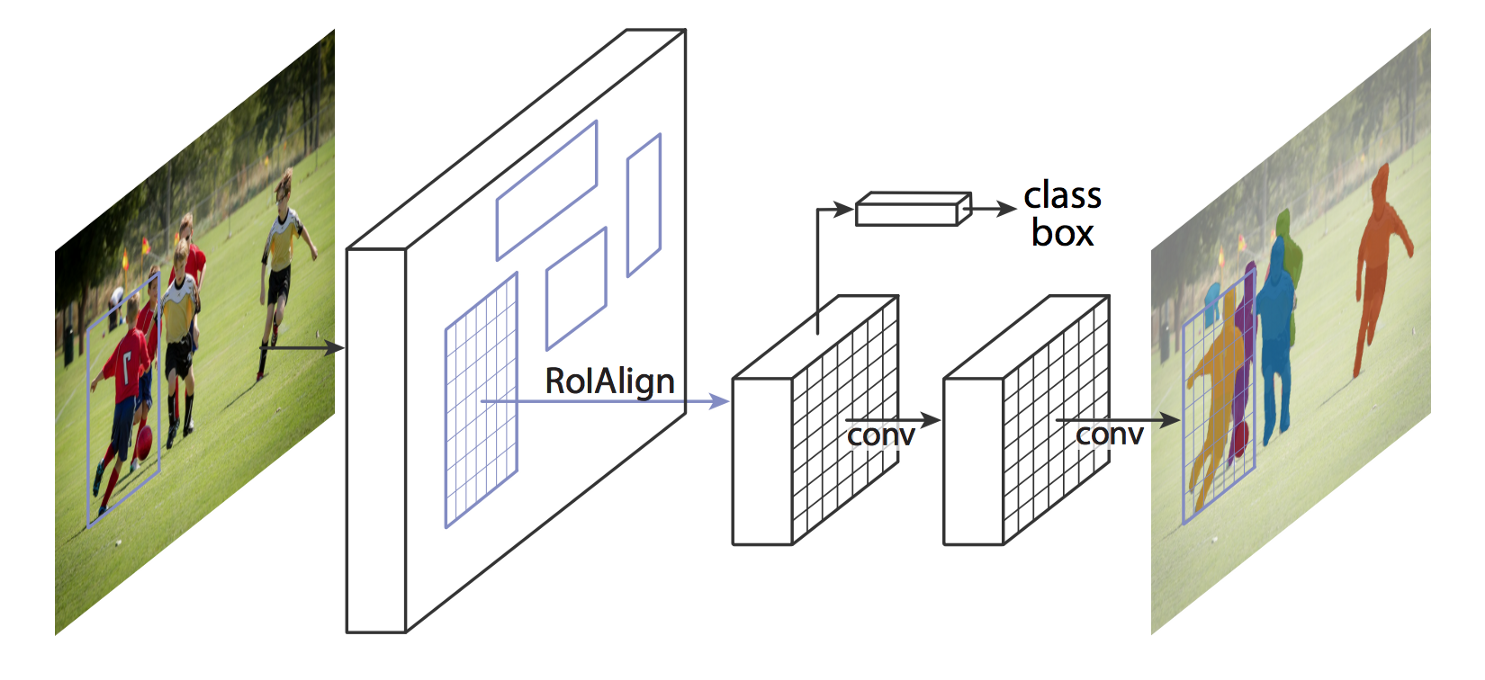
\includegraphics[width=0.5\linewidth]{PICs/maskrcnn.png}
 \caption{Mask R-CNN framework}
 \label{fig:maskRcnnFramework}
 \end{figure}


Like its predecessors, the Mask R-CNN \cite{He.op.2017} framework feeds the entire image to a \ac{CNN} and uses a Region Proposal Network to extract proposals from the feature map. Proposals from one feature map are then put together into one batch. Each proposal is cropped to the same size by RoI Align and then fed to a \acl{fc} network. The proposal is then classified by predicting a discrete probability for each k+1 probability, with the additional class being the background. Mask R-CNN takes a threshold between zero and one as hyper-parameter. If the probabilities fall under the threshold, the proposal is classified as background. Else, the object is localized while simultaneously the segmentation mask is predicted. 

The loss function L is a summation of three different factors:

\begin{equation} \label{lossFunction}   L= L_{cs} + L_{box} + L_{mask} \end{equation}

 \begin{itemize}
    \item \textbf{ \( \label{Lcs}L_{cs}\)} refers to the classification loss determined by the log loss function \( L_{cs}(p,u) = -log(p_{u})\). Mask R-CNN calculates a discrete probability \(p = (p_{0},...,p_{K})\), over K+1 classes, with the additional class being the background and the true class $u$.
    
    \item \textbf{ \( \label{Lbox}L_{box}\)} is defined over tuple $u,v=(v_{x},v_{y},v_{w},v_{h})$ with $v$ being a vector of bounding boxes for each class and the prediction $t=(t^{u}_{x},t^{u}_{y},t^{u}_{w},t^{u}_{h})$ with $u$ being the true class again. If $u$ is the background the $L_{box}$ is 0, otherwise 
    \begin{equation}
        L_{box}(t^{u},v)= \sum_{i \epsilon  \{x,y,w,h\}} smooth_{L_{1}}(t^{u}_{i} - v_{i})
    \end{equation}
    in which
    \begin{equation}
        smooth_{L_{1}}( s= t^{u}_{i} - v_{i})= 
\left\{\begin{matrix}
 0.5s^2 & if|s |<1 \\ |s|-0.5 & otherwise,
\end{matrix}\right.
    \end{equation}
    is a $L_{1}$ loss.
    
    \item \textbf{ \( \label{Lmask}L_{cs}\)} is similar to $L_{box}$ defined as average cross entropy loss. The predicted mask is compared to the ground truth.
\end{itemize}

Although Mask R-CNN predicts bounding boxes and mask for each class, only the losses of the true class from the ground truth contributes to the loss function. This decouples the mask prediction from the classification task. As a result, the mask branch can generate a mask for each class without competition among each other.
Each ROI acts as a sample and all ROI from an image are used as one mini batch. Mask R-CNN then uses Stochastic Gradient Descent \cite{Kiefer.1952}  to optimize the model.
%Barches and stochastic gardient
For details see \citetitle{Girshick.30Apr15} \cite{Girshick.30Apr15} and \citetitle{He.op.2017} \cite{He.op.2017}.






\chapter{Application } \label{Application}
As described in chapter \ref{Methodology}, the experiment is conducted with different CT images. These CT images are provided by \ac{SK}. \ac{SK} is a developer of the QDOSE Software \cite{.23Aug22}. The QDOSE Software is a dosimetry software used for individual
radiotherapy treatment planning. As part of the software, CT images are loaded and the organs are automatically segmented. Used images are gathered by \ac{SK} from public sources and used as training and validation data. 

\section{Data Description} \label{dataSescription}
    In total there are 210 different CT images and 210 label masks. Each image consists of approximately 216 slices with an average size of 512:512. For the experiment the traditional 75 to 25 train-test split was used, resulting in 158 CT images for training and 52 CT images for validation. The training data consists of 13127 slices containing a kidney for training, while the test images contain 2700 slices with a kidney. The values of the training and test data are not significantly different, which can be seen in Figure \ref{fig:data_desc}. Label masks are encoded with three different values:
    \begin{itemize}
        \item 0 for background
        \item 1 for kidney
        \item 2 for tumor
    \end{itemize}
 For the purpose of this thesis, tumors are ignored and treated as background with value zero. Both, CT images and label masks are provided in an NIfTI \cite{Brainder..2012,Knipe.2005} file format. 
    


 \begin{figure}
 \centering
 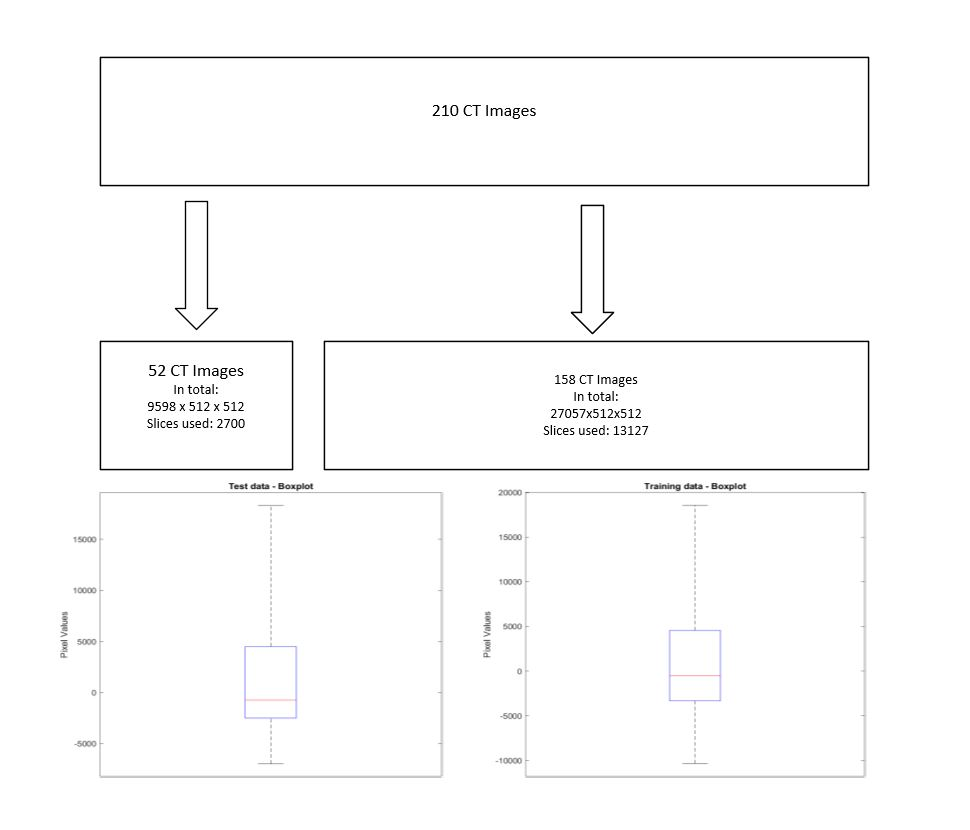
\includegraphics[width=0.7\linewidth]{PICs/data_desc.JPG}
 \caption{Data description - \textit{Test data:} Min: -6986, 1st: -1001, Median: -744, 3rd: -110, Max: 18326, Var: 348110; 
 \textit{Training data:} Min: -10240, 1st: -1003, Median: -540, 3rd: -109, Max: 18558, Var: 305240 }
 \label{fig:data_desc}
 \end{figure}



\section{Experiment} \label{Experiment}
The network was trained with following environment:

\begin{description}
    \item OS Microsoft Windows 10 Education~Version	10.0.19044
    \item CPU Intel(R) Core(TM) i7-7700 CPU @ 3.60GHz  
    \item RAM  16,0 GB
    \item GPU  NVIDIA GeForce GTX 1080 Ti                         
\end{description}

Before training, the training images described in chapter \ref{dataSescription} were normalized to reach a value between zero and one. In total, the network is trained over ten epochs. Each epoch consisted of 13127 steps over approximately 6 hours, resulting into a total training time of 60 hours. The Matlab Mask R-CNN implementation \cite{GitHub.25Aug22, .25Aug22} uses a ResNet50 \cite{K.He.2016}  backbone and allows to set up a threshold as described in chapter \ref{MaskRCNN}. With the threshold it is possible to increase and decrease the amount of false positive/negative. For the experiment, each of the ten networks was validated against the test data with ten different thresholds ranging from 0.1 to 1.0 with an interval of 0.1. As Mask R-CNN adjust the mini batch size automatically as described in chapter \ref{MaskRCNN}, no batch size is given.
Results can be seen in chapter \ref{Results}. Used metrics are described in chapter \ref{Methodology}.
 



\section{Results and Discussion} \label{Results}
Each network was tested with ten different thresholds against 52 CT images using the metrics described in chapter \ref{Experiment}. For the sake of simplicity, the results from the 52 CT images are taken as a mean in figure \ref{fig:MeanValues}.
\begin{figure*}
        \centering
        \begin{subfigure}[b]{0.475\textwidth}
            \centering
            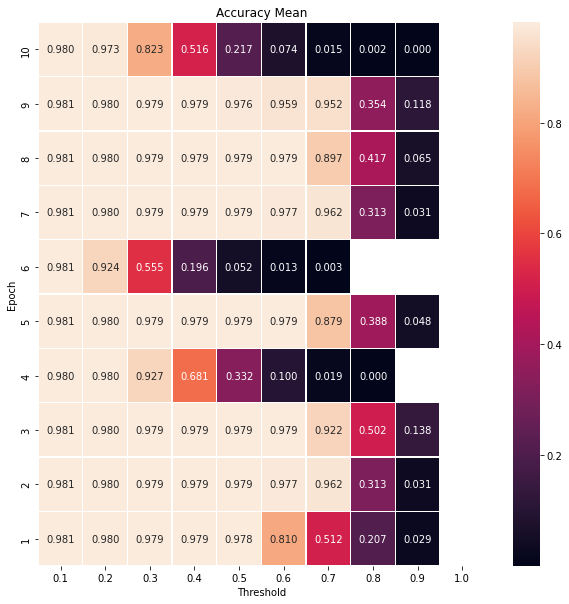
\includegraphics[width=\textwidth]{PICs/accuracy_mean.png}
            \caption[Accuracy Mean]%
            {{\small Accuracy Mean}}    
            \label{fig:acMean}
        \end{subfigure}
        \hfill
        \begin{subfigure}[b]{0.475\textwidth}  
            \centering 
            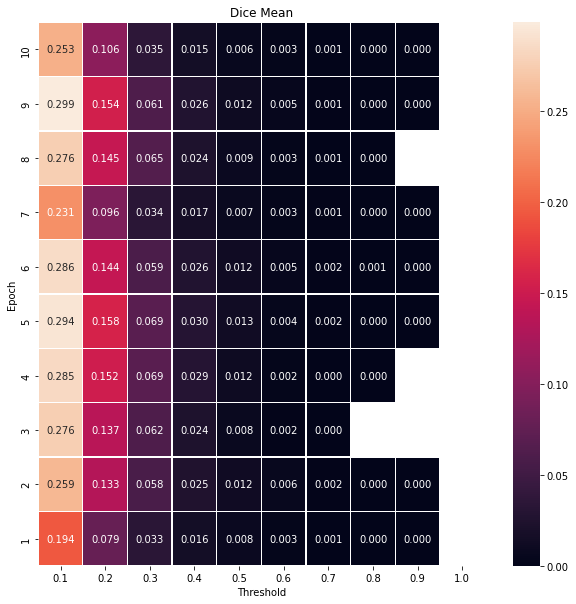
\includegraphics[width=\textwidth]{PICs/dice_mean.png}
            \caption[Dice Coefficient Mean]%
            {{\small Dice Coefficient Mean}}    
            \label{fig:diceMean}
        \end{subfigure}
        \vskip\baselineskip
        \begin{subfigure}[b]{0.475\textwidth}   
            \centering 
            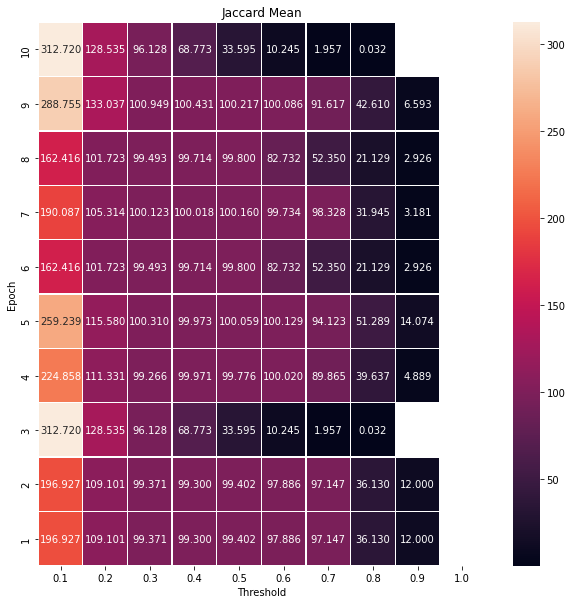
\includegraphics[width=\textwidth]{PICs/jaccard_mean.png}
            \caption[Jaccard Index Mean]%
            {{\small Jaccard Index Mean}}    
            \label{fig:jMean}
        \end{subfigure}
        \hfill
        \begin{subfigure}[b]{0.475\textwidth}   
            \centering 
            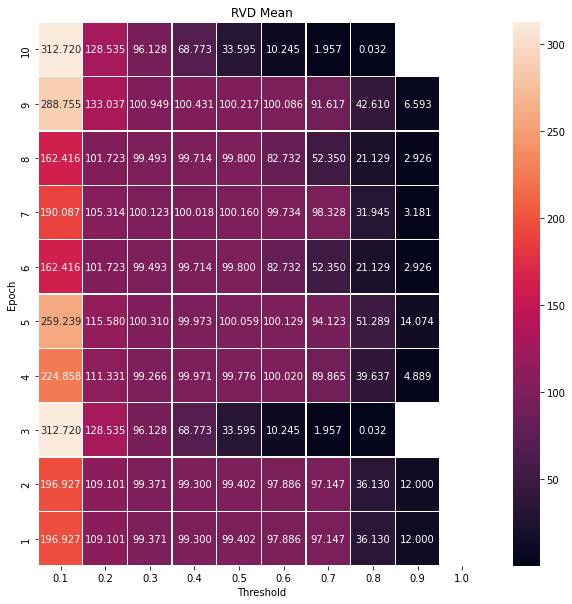
\includegraphics[width=\textwidth]{PICs/rvd_mean.png}
            \caption[RVD Mean]%
            {{\small RVD Mean}}    
            \label{fig:rvdMean}
        \end{subfigure}
        \caption[ Mean Average, Dice Coefficient, Jaccard Index and RVD for each epoch from one to ten and threshold 0.1 to 1.0 ]
        {\small Mean Average, Dice Coefficient, Jaccard Index and RVD for each epoch from one to ten and threshold 0.1 to 1.0} 
        \label{fig:MeanValues}
    \end{figure*}
    
The results displayed in figure \ref{fig:MeanValues} indicate greater results on a lower threshold, which deteriorate as the threshold increases. The performance drops significantly when the threshold reaches 0.5. Noticeably, the \ac{DSC} performs worse than the accuracy. This indicates a large unbalance between the amount of background and kidney pixels. An example can be seen in figure \ref{fig:kidneyMask}, where the green prediction mask is more than twice the size of the pink ground truth is more than double in size. Additionally, the kidney is also small, compared to the rest of the background.

 \begin{figure}
 \centering
 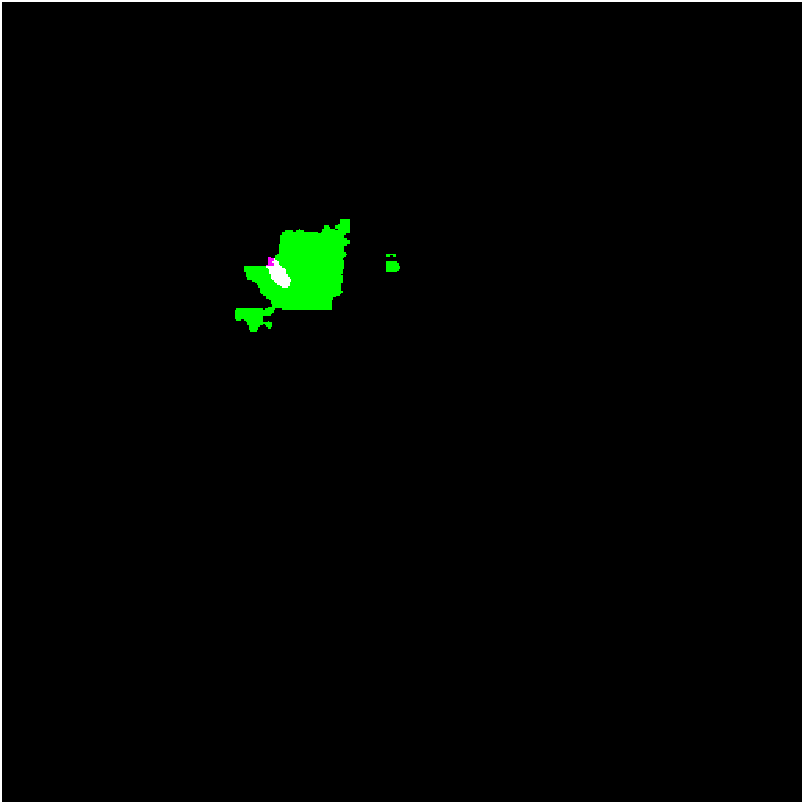
\includegraphics[width=0.3\linewidth]{PICs/kidneyMask.png}
 \caption{Prediction over ground truth label - Pink: kidney label; Green: prediction mask}
 \label{fig:kidneyMask}
 \end{figure}
 
 
For further analyzation, results using the network of epoch five and an 0.5 threshold were grouped by CT image and taken as a mean, in order to display  the performance of  the model for the different parts of the kidney (see figure \ref{fig:align}).
 \begin{figure}
 \centering
 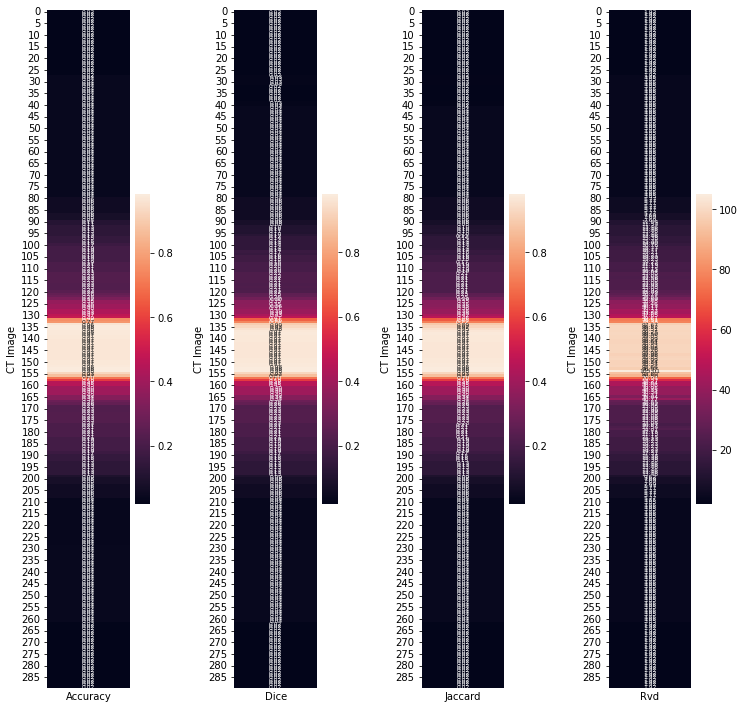
\includegraphics[width=0.5\linewidth]{PICs/align.png}
 \caption{Epoch: 5, Threshold: 0.5 - Mean  Accuracy, Jaccard Index, Dice Coefficient and RVD from top to bottom}
 \label{fig:align}
 \end{figure}
 
 The volume distribution can be seen in figure \ref{fig:volumeDistribution}. Details are attached at the end of the thesis.
 \begin{figure}[!htbp]
 \centering
 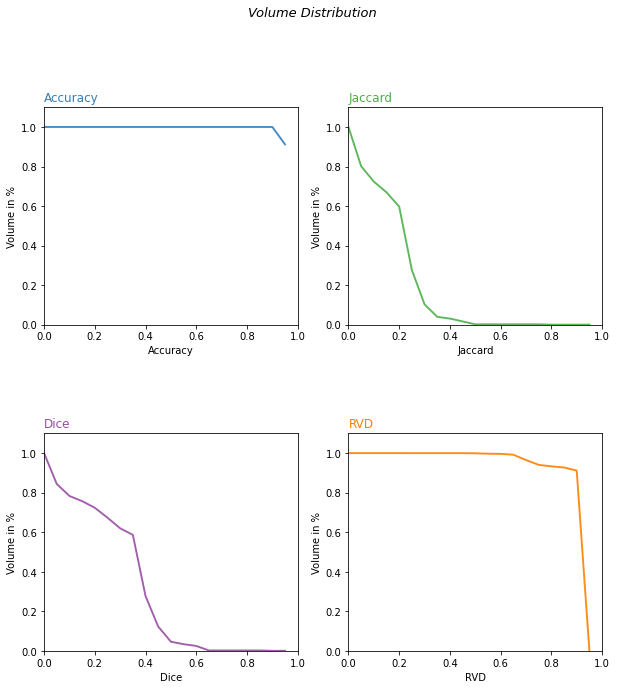
\includegraphics[width=0.9\linewidth]{PICs/volumeDistibution.png}
 \caption{Volume Distribution for Accuracy, Jaccard Index, Dice Coefficient and RVD  - epoch 5, threshold 0.5, RVD $10^{-2}$ }
 \label{fig:volumeDistribution}
 \end{figure}
\ac{J}, \ac{DSC} and \ac{RVD} in figure \ref{fig:volumeDistribution} show low performance while \ac{AC} being the only positive indicator. \ac{J} and \ac{DSC} display low congruence with the expert segmentation while \ac{RVD} indicate large differences between prediction and actual segmentation. The visualization of figure \ref{fig:align} clearly shows a better performance in the middle part of the kidney, where it has a more regular and balanced form than at the top or bottom, where unbalanced data is to be expected. This leads to the conclusion, that Mask R-CNN is able to segment objects of a class if the form and size does not change but fails if otherwise. In regards to the research questions, it can be concluded that it is not feasible to train Mask R-CNN for automated kidney segmentation because of the low congruence with expert segmentation. With a segmentation time of approximately 0.1254 seconds per slice or 6.4464 seconds per CT image, the model is fast enough for practical usage, but based on the other metrics, it is not advised. 
%Limitation 
Nevertheless, this conclusion is based on the given data and the usage of a 2D Mask R-CNN implementation of Matlab \cite{GitHub.25Aug22, .25Aug22}. Although papers as "\citetitle{Vuola.29Jan19}" \cite{Vuola.29Jan19}  and   \citetitle{OvergaardLauersen.2021} \cite{OvergaardLauersen.2021} display the shortcomings of Mask R-CNN with organic images and describe tasks such as kidney segmentation as challenging, different papers suggest better results or improvements. As an example, in \citetitle{Goyal.2022} \cite{Goyal.2022} the framework reaches a \ac{DSC} of 90,5\% and a \ac{J} of 82,8 \%, while other papers \cite{Chen., Shu.2020} reach metrics significantly above 90\%  by developing the framework even further. 
One of the suggested developments was the change from a two dimensional ROI Align to a three dimensional ROI Align algorithm. Another paper, \citetitle{Nazari.2021} \cite{Nazari.2021}, uses a similar approach to reach a better performance.  Even though the aggregated results indicate low performance, they also show high \ac{AC} with low \ac{DSC}. This is typical for unbalance data as described above. This supports the theory for the need of further research by improving the current framework.


\chapter{Conclusion} \label{Conclusion}
This thesis is an additional contribution that shows the limitations of Mask R-CNN on a two dimensional plane. Although the framework is proven to be efficient with natural images, segmentation on biological images is still a challenge. Mask R-CNN is sufficient if the object has a consistent shape on a two dimensional plane, but not if it varies.  As the later circumstance is common with organs, it is not feasible to use Mask R-CNN with a two-dimensional ROI Align for organ segmentation. As described in chapter \ref{Results}, other papers support this statement. Nevertheless, the papers also indicate potential improvement by further developing the current Mask R-CNN model. Furthermore, this thesis only uses only a limited amount of data and is bound to the implementation of Matlab. This has to be considered when evaluating the impact of this study. 



\clearpage
\printbibliography
\clearpage

% Das Abbildungsverzeichnis
\listoffigures
\clearpage

% Das Tabellenverzeichnis
%\listoftables
\clearpage

% Das Quellcodeverzeichnis
%\listofcode
\clearpage

\phantomsection

\addcontentsline{toc}{chapter}{\listacroname}
\chapter*{\listacroname}
\begin{acronym}[XXXXX]
    \acro{AC} { Accuracy}
    \acro{AI}[AI]{Artificial Intelligence}
    \acro{ANN}[ANN]{Artificial Neural Network}
    \acro{CT}[CT]{Computed Tomography}
    \acro{CNN}[CNN]{Convolutional Neural Network}
    \acro{DSC} {Sørensen–Dice Coefficient}
    \acro{fc}[fc]{fully connected}
    \acro{GDPR} {General Data Protection Regulation}
    \acro{HDD} {Hausdorff Distance}
    \acro{IoU} {Intersection over Union}
    \acro{J} {Jaccard Index}
    \acro{MRT} {molecular radiotherapy}
    \acro{OAR}{Organ at Risk}
    \acro{RoI}[RoI]{Region of Interests}
    \acro{RVD}{ Relative Volume Difference}
    \acro{SVM}[SVM]{Support Vector Machine}
    \acro{SK}{Sharok Kimiaei} 
\end{acronym}


%
% Hier beginnt der Anhang.
%
\clearpage
\appendix
\chapter{Anhang - Detailed results}
 \begin{figure}[!htbp]
 \centering
 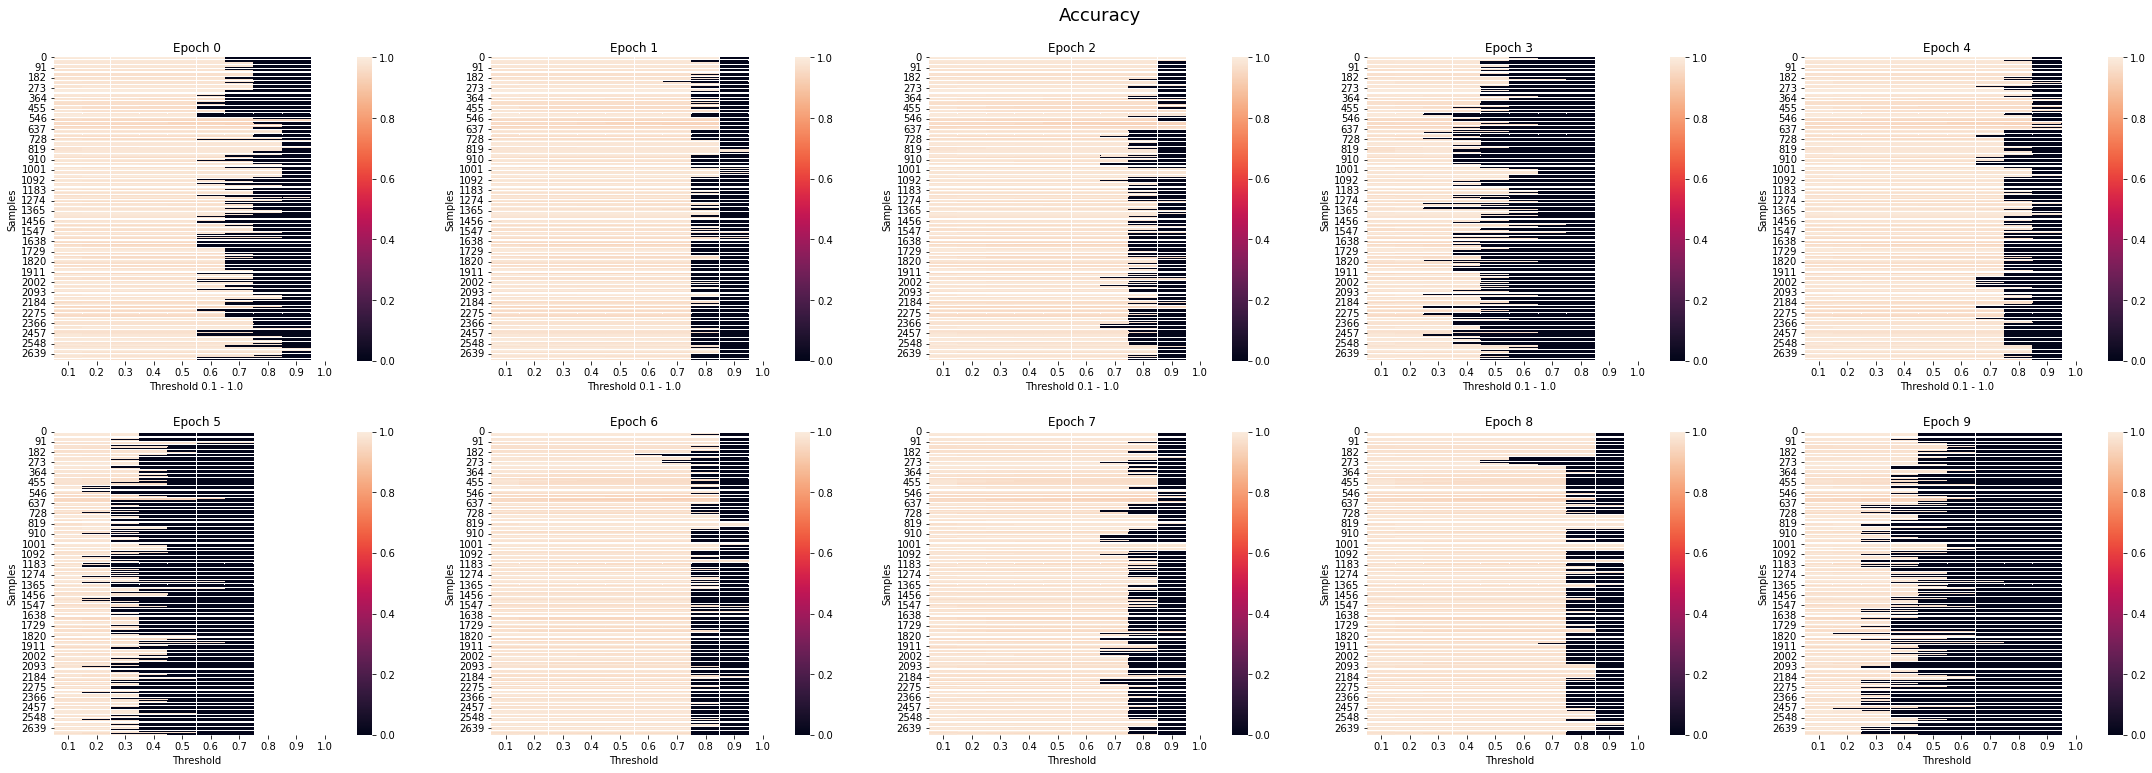
\includegraphics[width=1\linewidth]{PICs/accuracy.png}
 \caption{Accuracy per epoch, threshold and sample}
 \label{fig:accuracy}
 \end{figure}


 \begin{figure}[!htbp]
 \centering
 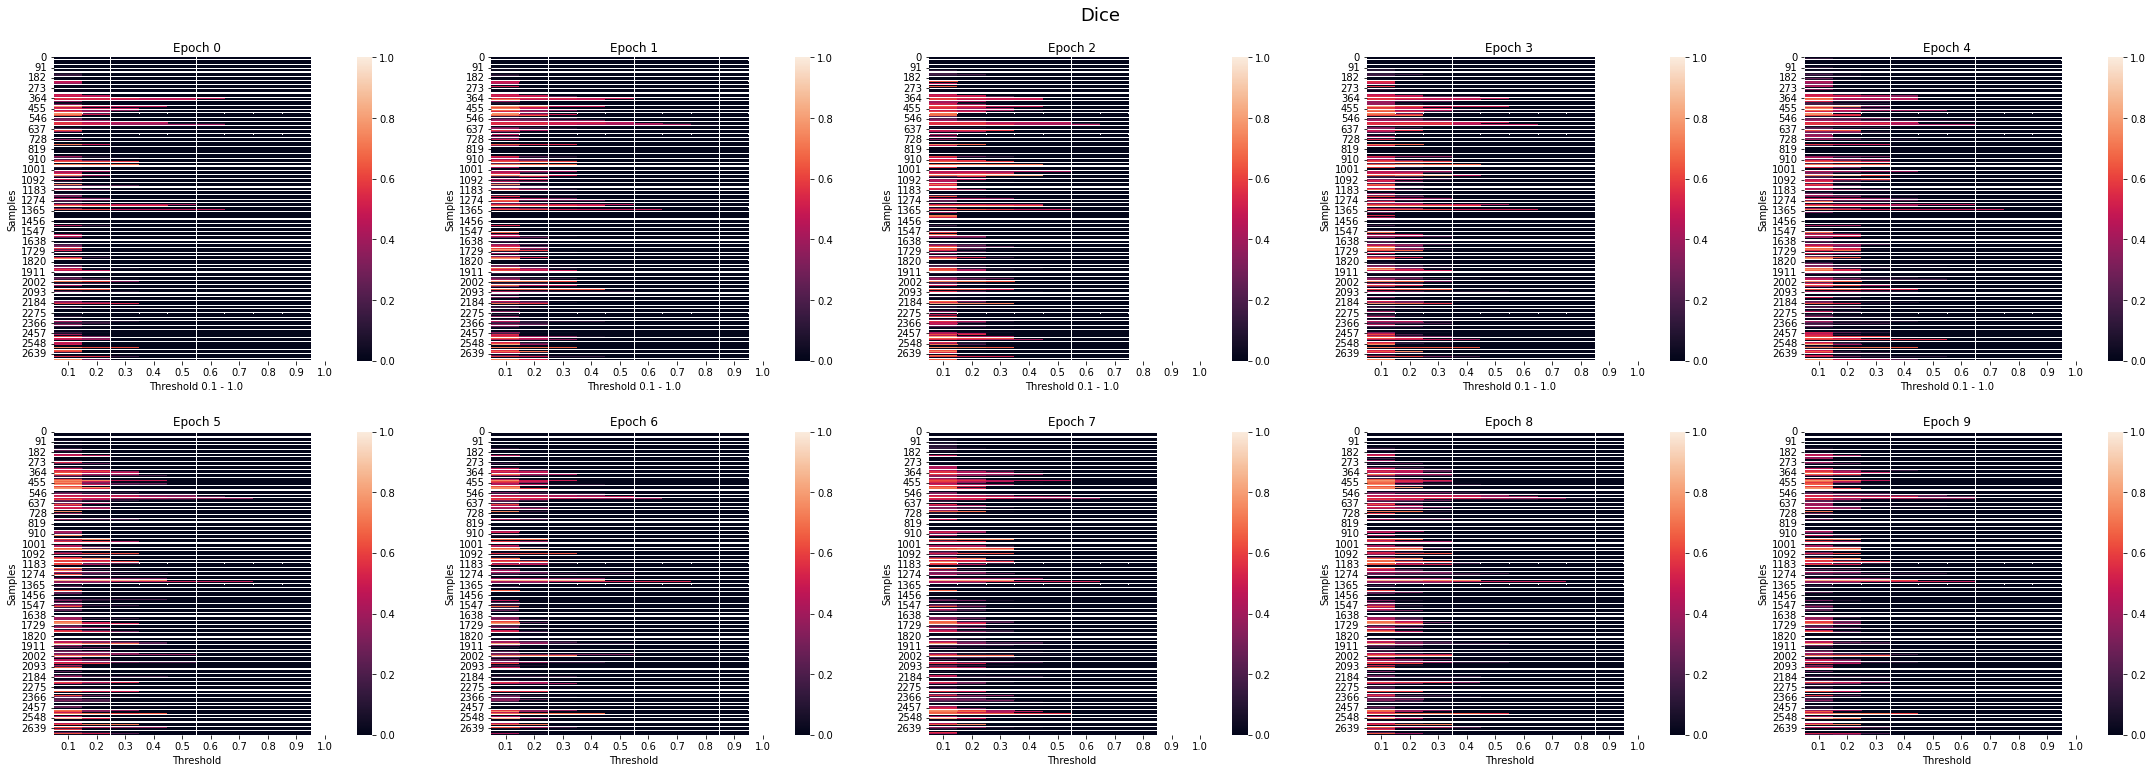
\includegraphics[width=1\linewidth]{PICs/dice.png}
 \caption{Dice Coefficient per epoch, threshold and sample}
 \label{fig:dice}
 \end{figure}



 \begin{figure}[!htbp]
 \centering
 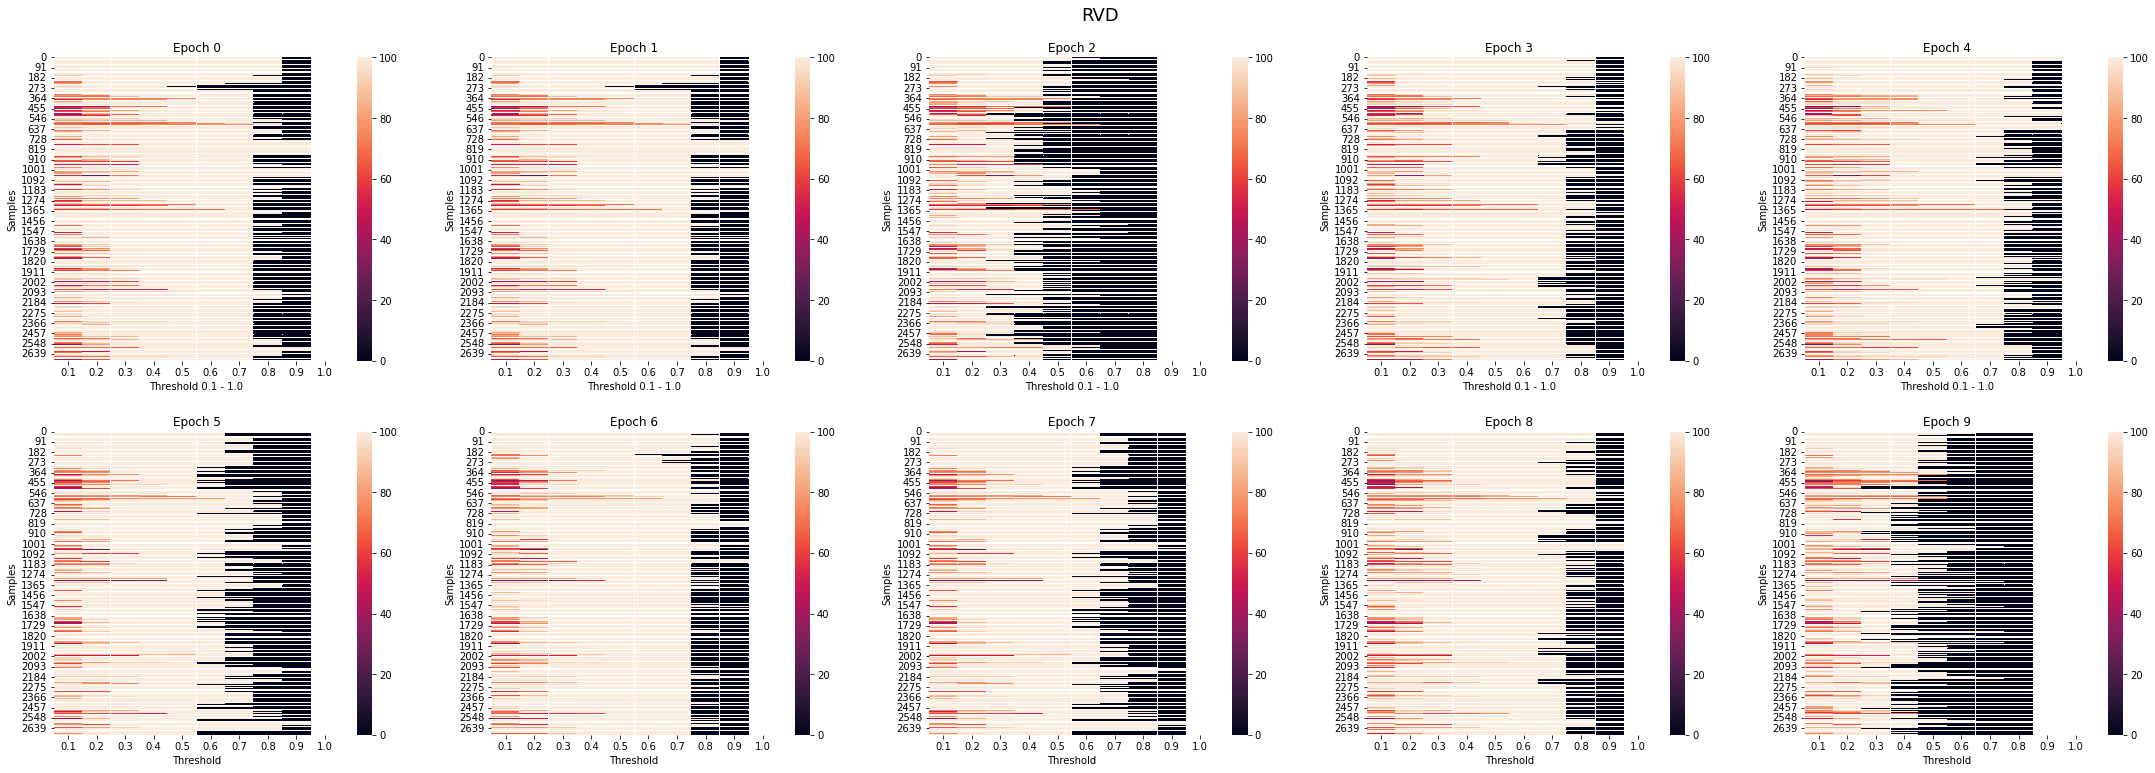
\includegraphics[width=1\linewidth]{PICs/rvd.png}
 \caption{RVD per epoch, threshold and sample}
 \label{fig:rvd}
 \end{figure}



 \begin{figure}[!htbp]
 \centering
 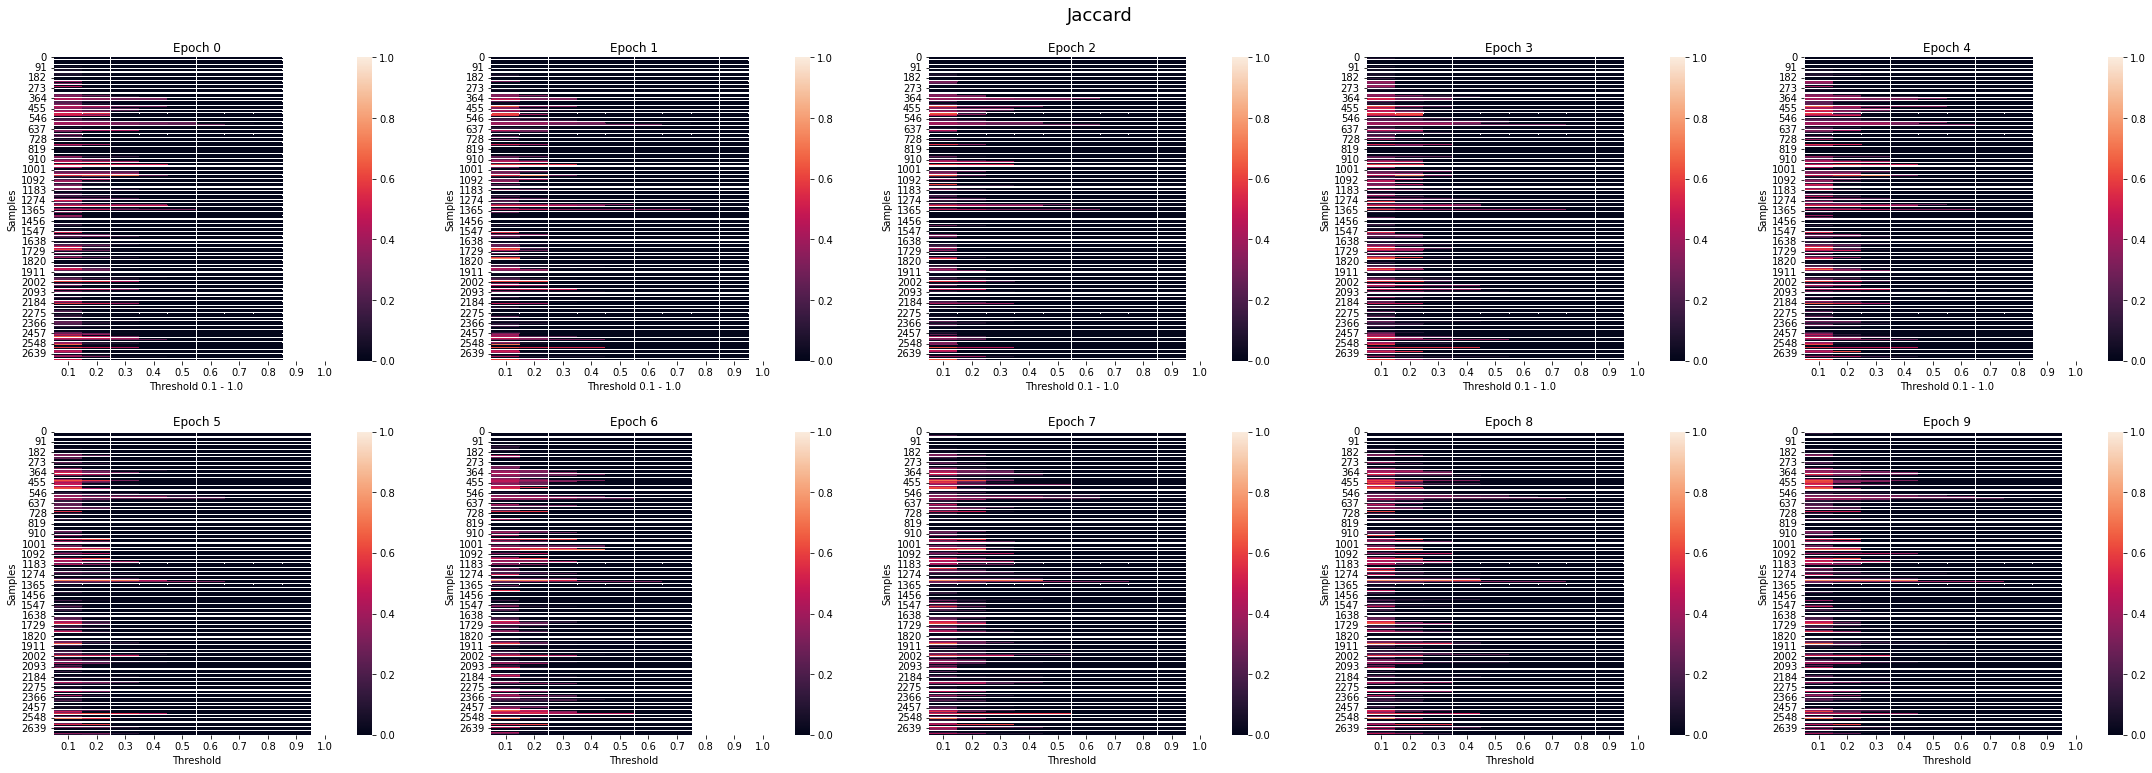
\includegraphics[width=1\linewidth]{PICs/jaccard.png}
 \caption{Jaccard Index per epoch, threshold and sample}
 \label{fig:accuracy}
 \end{figure}

\clearpage
\chapter{Anhang - Code}
All Code and data can also be found on  \url{https://github.com/Codo155/maskRcnn_Msc}

\section{Matlab Code}


\definecolor{mygreen}{RGB}{28,172,0} % color values Red, Green, Blue
\definecolor{mylilas}{RGB}{170,55,241}



\lstset{language=Matlab,%
    %basicstyle=\color{red},
    breaklines=true,%
    morekeywords={matlab2tikz},
    keywordstyle=\color{blue},%
    morekeywords=[2]{1}, keywordstyle=[2]{\color{black}},
    identifierstyle=\color{black},%
    stringstyle=\color{mylilas},
    commentstyle=\color{mygreen},%
    showstringspaces=false,%without this there will be a symbol in the places where there is a space
    numbers=left,%
    numberstyle={\tiny \color{black}},% size of the numbers
    numbersep=9pt, % this defines how far the numbers are from the text
    emph=[1]{for,end,break},emphstyle=[1]\color{red}, %some words to emphasise
    %emph=[2]{word1,word2}, emphstyle=[2]{style},    
}


\section*{Matlab Code}

\lstinputlisting{Code/getCoordinates.m}
\lstinputlisting{Code/maskRcnn.m}
\lstinputlisting{Code/normalization.m}
\lstinputlisting{Code/speedTest.m}
\lstinputlisting{Code/validateAlignKidney.m}
\lstinputlisting{Code/validation.m}
\lstinputlisting{Code/validationFunction.m}
\lstinputlisting{Code/validateKidneyVolumeHistogram.m}
\newcommand\invisiblesection[1]{%
  \refstepcounter{section}%
  \addcontentsline{toc}{section}{\protect\numberline{\thesection}#1}%
  \sectionmark{#1}}
\invisiblesection{Python visual analyzation of results}

\end{document}
